% 用 XeLaTeX 编译；ctex 会按系统自动选择中文字体。
\documentclass[UTF8,zihao=-4]{ctexart}
\usepackage[a4paper,margin=2.5cm]{geometry}
\usepackage{amsmath,amssymb}
\usepackage{graphicx}
\usepackage{booktabs}
\usepackage[numbers,sort&compress]{natbib}
\usepackage[colorlinks=true,allcolors=blue]{hyperref}

\title{论文题目}
\author{作者一\thanks{单位，\texttt{author@example.edu.cn}} \and 作者二}
\date{\today}

\begin{document}
\maketitle

\begin{abstract}
用两三百字概括研究问题、方法、主要结果和意义。
\end{abstract}

\section{引言}
\label{sec:intro}
介绍研究背景与现有工作的不足\cite{knuth1984,lamport1994}。
第~\ref{sec:method}~节介绍方法，第~\ref{sec:results}~节给出结果。

\section{方法}
\label{sec:method}
定义所用的物理量，例如吉布斯自由能
\begin{equation}
  \label{eq:energy}
  G = H - TS ,
\end{equation}
其中 $H$ 为焓，$T$ 为温度，$S$ 为熵。

\section{结果}
\label{sec:results}
图~\ref{fig:example} 和表~\ref{tab:example} 汇总了主要结果。

\begin{figure}[htbp]
  \centering
  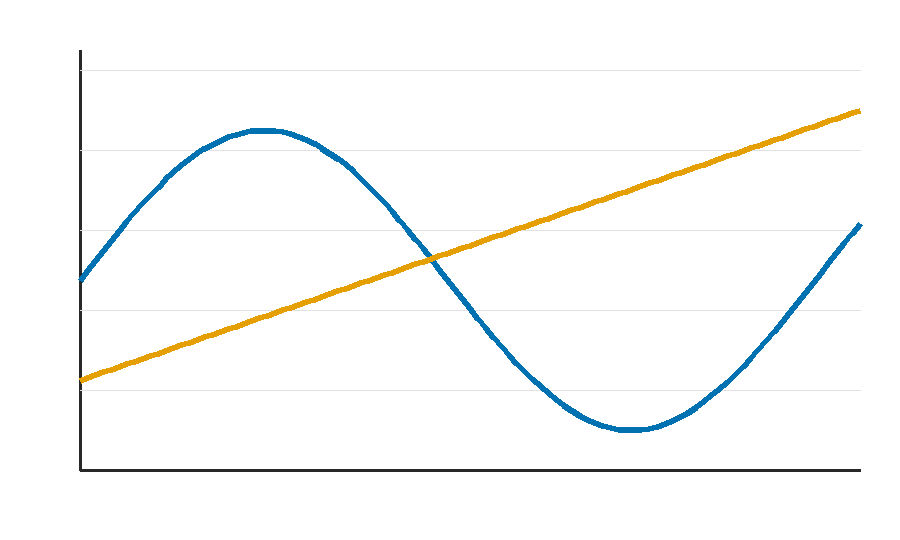
\includegraphics[width=0.6\linewidth]{figures/example.png}
  \caption{示例图，请替换为自己的图片并放在 figures 文件夹中。}
  \label{fig:example}
\end{figure}

\begin{table}[htbp]
  \centering
  \caption{示例表格}
  \label{tab:example}
  \begin{tabular}{lcc}
    \toprule
    样品 & 指标 A & 指标 B \\
    \midrule
    S1 & 1.00 & 2.00 \\
    S2 & 1.50 & 2.50 \\
    \bottomrule
  \end{tabular}
\end{table}

\section{结论}
总结主要发现和后续工作。

\bibliographystyle{unsrtnat}
\bibliography{refs}

\end{document}
